\documentclass[]{article}
\usepackage{lmodern}
\usepackage{amssymb,amsmath}
\usepackage{ifxetex,ifluatex}
\usepackage{fixltx2e} % provides \textsubscript
\ifnum 0\ifxetex 1\fi\ifluatex 1\fi=0 % if pdftex
  \usepackage[T1]{fontenc}
  \usepackage[utf8]{inputenc}
\else % if luatex or xelatex
  \ifxetex
    \usepackage{mathspec}
  \else
    \usepackage{fontspec}
  \fi
  \defaultfontfeatures{Ligatures=TeX,Scale=MatchLowercase}
\fi
% use upquote if available, for straight quotes in verbatim environments
\IfFileExists{upquote.sty}{\usepackage{upquote}}{}
% use microtype if available
\IfFileExists{microtype.sty}{%
\usepackage{microtype}
\UseMicrotypeSet[protrusion]{basicmath} % disable protrusion for tt fonts
}{}
\usepackage[margin=1in]{geometry}
\usepackage{hyperref}
\PassOptionsToPackage{usenames,dvipsnames}{color} % color is loaded by hyperref
\hypersetup{unicode=true,
            pdftitle={Lab01},
            pdfauthor={Patrick Bitterman},
            colorlinks=true,
            linkcolor=Maroon,
            citecolor=Blue,
            urlcolor=Blue,
            breaklinks=true}
\urlstyle{same}  % don't use monospace font for urls
\usepackage{graphicx,grffile}
\makeatletter
\def\maxwidth{\ifdim\Gin@nat@width>\linewidth\linewidth\else\Gin@nat@width\fi}
\def\maxheight{\ifdim\Gin@nat@height>\textheight\textheight\else\Gin@nat@height\fi}
\makeatother
% Scale images if necessary, so that they will not overflow the page
% margins by default, and it is still possible to overwrite the defaults
% using explicit options in \includegraphics[width, height, ...]{}
\setkeys{Gin}{width=\maxwidth,height=\maxheight,keepaspectratio}
\IfFileExists{parskip.sty}{%
\usepackage{parskip}
}{% else
\setlength{\parindent}{0pt}
\setlength{\parskip}{6pt plus 2pt minus 1pt}
}
\setlength{\emergencystretch}{3em}  % prevent overfull lines
\providecommand{\tightlist}{%
  \setlength{\itemsep}{0pt}\setlength{\parskip}{0pt}}
\setcounter{secnumdepth}{0}
% Redefines (sub)paragraphs to behave more like sections
\ifx\paragraph\undefined\else
\let\oldparagraph\paragraph
\renewcommand{\paragraph}[1]{\oldparagraph{#1}\mbox{}}
\fi
\ifx\subparagraph\undefined\else
\let\oldsubparagraph\subparagraph
\renewcommand{\subparagraph}[1]{\oldsubparagraph{#1}\mbox{}}
\fi

%%% Use protect on footnotes to avoid problems with footnotes in titles
\let\rmarkdownfootnote\footnote%
\def\footnote{\protect\rmarkdownfootnote}


  \title{Lab01}
    \author{Patrick Bitterman}
      \date{1/30/2021}


% change section title styling
\usepackage{sectsty}
\sectionfont{\normalsize\normalfont\itshape}
\subsectionfont{\normalsize\normalfont}

% use fancyhdr style
\usepackage{fancyhdr}
\pagestyle{fancy}
\fancyhead[LO, LE]{Lab01}
\fancyhead[RO, RE]{GEOG 432/832}
\makeatletter
\renewcommand{\maketitle}{\bgroup\vspace*{-1cm}\setlength{\parindent}{0pt}
\begin{flushleft}
  \@author
  
  \@date
  
\end{flushleft}\egroup
}
\makeatother

\begin{document}
\maketitle

\hypertarget{lab-01-python-fundamentals-and-geoprocessing-in-arcgis-pro}{%
\section{Lab 01: Python fundamentals and geoprocessing in ArcGIS
Pro}\label{lab-01-python-fundamentals-and-geoprocessing-in-arcgis-pro}}

\hypertarget{read-the-instructions-completely-before-starting-the-lab}{%
\subsubsection{Read the instructions COMPLETELY before starting the
lab}\label{read-the-instructions-completely-before-starting-the-lab}}

\hypertarget{part-1-python-fundamentals}{%
\subsection{Part 1: Python
fundamentals}\label{part-1-python-fundamentals}}

The purpose of part 1 is to (re-)introduce you to basic Python
functionality and to demonstrate functions that we don't cover in class.
Because students have varying levels of experience with Python, I have
provided the lab exercise from your textbook as a refresher. This file
is named \emph{``PythonScripting\_Ex04.pdf''}. You may complete as much
or as little of the exercises as you like, depending on your experience
and comfort with Python. This lab assumes you have read Chapter 4 from
your textbook. For Part 1, you may use whatever editor/interpreter you
wish (e.g., Jupyter, Spyder, IDLE)

\hypertarget{for-part-1-you-must-write-and-turn-in-scripts-that-complete-the-following-tasks}{%
\subsubsection{For part 1, you must write and turn in script(s) that
complete the following
tasks:}\label{for-part-1-you-must-write-and-turn-in-scripts-that-complete-the-following-tasks}}

\begin{enumerate}
\def\labelenumi{\arabic{enumi}.}
\item
  Extracts the sub-string ``GIScience'' from the String ``Learning
  GIScience is awesome!''
\item
  Uses a loop control structure to count from 0-100 by fives. The script
  should print the value to the console AND should print whether the
  value is odd or even. For example, an output could look like ``15 is
  odd''
\item
  Calculates and prints (with meaningful statements) the sum, median,
  and mean of the array {[}7, 24.5, 99, 101, 256, 128, 1000{]}. You must
  use array references or other functions in the math - do NOT directly
  use the numeric values in the calculation. The code should be general
  enough to perform the calculations for any given array. Test the same
  code using the array {[}1, 2, 3, 4, 5{]}. Show both results.
\item
  Reads the ``lab01textsample.txt'' file, assigns it to a variable, and
  then prints the file line-by-line. Extra points if you can skip
  printing the first 2 lines.
\item
  Write a function that accepts as a parameter a numeric value
  corresponding to the \textbf{percentage score} for the class and and
  returns the corresponding letter grade for the course. It must also
  return an appropriate message for scores outside of the correct range
  of scores. You don't have to bother with pluses or minuses, just full
  letter grades. Finally, test your function and show that it works for
  the scores: -5, 45, 70, 99, and 125.
\end{enumerate}

\newpage

\hypertarget{part-2-modeling-precipitation-zones-in-nebraska-in-arcgis-pro}{%
\subsection{Part 2: Modeling precipitation zones in Nebraska in ArcGIS
Pro}\label{part-2-modeling-precipitation-zones-in-nebraska-in-arcgis-pro}}

Suppose you're working on a project for the Nebraska Department of
Agriculture and you are tasked with making some maps of precipitation in
the state. Members of the department want to see which parts of the
state were relatively dry and wet in the past year, classified in zones.
All you have is a series of weather station readings of cumulative
rainfall for 2008 that you've obtained from within Nebraska and
surrounding areas. This is a shapefile of points called
Precip2008Readings.shp. It is in your lab01 data folder.

Precip2008Readings.shp is a fictional dataset created for this project.
The locations do not correspond to actual weather stations. However, the
measurements are derived from real 2018 precipitation data created by
the PRISM Climate Group at Oregon State University, 2019.

You need to do several tasks in order to get this data ready for
mapping:

\begin{itemize}
\tightlist
\item
  Interpolate a precipitation surface from your points. This creates a
  raster dataset with estimated precipitation values for your entire
  area of interest. You've already planned for this, knowing that you
  are going to use inverse distance weighted (IDW) interpolation. Click
  the following link to learn how the IDW technique works.
\end{itemize}

\url{https://pro.arcgis.com/en/pro-app/latest/tool-reference/3d-analyst/how-idw-works.htm}

You've also selected your points to include some areas around Nebraska
to avoid edge effects in the interpolation.

\begin{itemize}
\item
  Reclassify the interpolated surface into an ordinal classification of
  precipitation ``zones'' that delineate relatively dry, medium, and wet
  regions.
\item
  Create vector polygons from the zones.
\item
  Clip the zone polygons to the boundary of Nebraska.
\end{itemize}

\begin{figure}
\centering
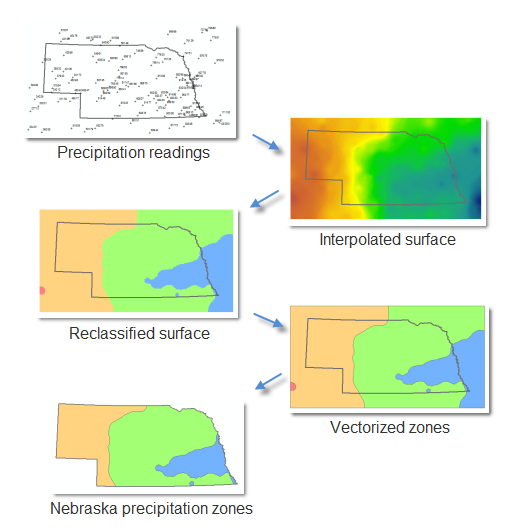
\includegraphics{./labs/images/project1_model_workflow.png}
\caption{Generalized workflow}
\end{figure}

It's very possible that you'll want to repeat the above process in order
to test different IDW interpolation parameters or make similar maps with
other datasets (such as next year's precipitation data). Therefore, the
above series of tasks is well-suited to ModelBuilder. Your job is to
create a model that can complete the above series of steps without you
having to manually open four different tools.

Model parameters Your model should have these (and only these)
parameters:

\begin{enumerate}
\def\labelenumi{\arabic{enumi}.}
\item
  Input precipitation readings- This is the location of your
  precipitation readings point data. This is a model parameter so that
  the model can be easily re-run with other datasets.
\item
  Power- An IDW setting specifying how quickly influence of surrounding
  points decreases as you move away from the point to be interpolated.
\item
  Search radius- An IDW setting determining how many surrounding points
  are included in the interpolation of a point. The search radius can be
  fixed at a certain distance, including whatever number of points
  happen to fall within, or its distance can vary in order for it to
  always include a minimum number of points. When you use ModelBuilder,
  you don't have to set up any of these choices; ModelBuilder does it
  for you when you set the Search Radius as a model parameter.
\item
  Zone boundaries- This is a table allowing the user of the model to
  specify the zone boundaries. For example, you could configure
  precipitation values of 0 - 30000 to result in a reclassification of 1
  (to correspond with Zone 1), 30000 - 60000 could result in a
  classification of 2 (to correspond with Zone 2), and so on. The way to
  get this table is to make a variable from the Reclassification
  parameter of the Reclassify tool and set it as a model parameter.
\item
  Output precipitation zones- This is the location where you want the
  output dataset of clipped vector zones to be placed on disk.
\end{enumerate}

As you build your model, you will need to configure some settings that
will not be exposed as parameters. These include the clip feature, which
is the state of Nebraska outline Nebraska.shp in your lab01 data folder.
There are many other settings such as ``Z Value field'' and ``Input
barrier polyline features'' (for IDW) or ``Reclass field'' (for
Reclassify) that should not be exposed as parameters. You should just
set these values once when you build your model. If you ever ask someone
else to run this model, you don't want them to be overwhelmed with
choices stemming from every tool in the model; you should just expose
the essential things they might want to change.

For this particular model, you should assume that any input dataset will
conform to the same schema as your Precip2008Readings.shp feature class.
For example, an analyst should be able to submit a similar
Precip2009Readings dataset with the same fields, field names, and data
types. However, he or she should not expect to provide any feature class
with a different set of fields and field names, etc. As you might
discover, handling all types of feature class schemas would make your
model more complex than we want for this assignment.

When you double-click the model to run it, the interface should look
like the following:

\begin{figure}
\centering
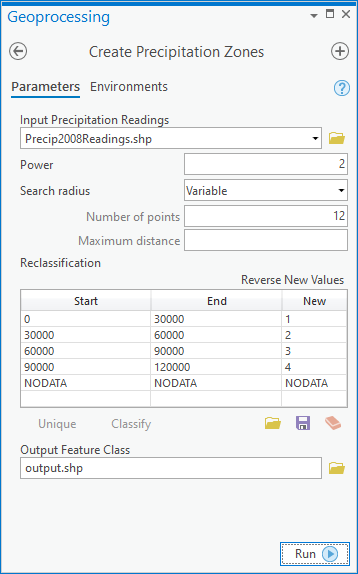
\includegraphics{./labs/images/create_precip_zones_ui_pro_0.png}
\caption{Model parameters dialog}
\end{figure}

Running the model with the exact parameters listed above should result
in the following (the zones have been symbolized with different colors
to help distinguish them). This is one way you can check your work:

\begin{figure}
\centering
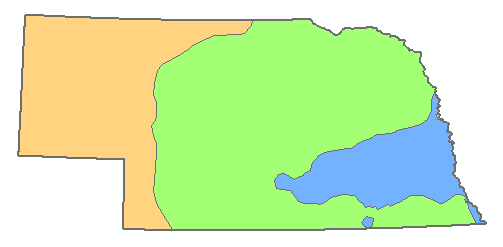
\includegraphics{./labs/images/project1_model_output.png}
\caption{Model Output}
\end{figure}

\hypertarget{tips}{%
\subsubsection{Tips}\label{tips}}

The following tips may help you as you build your model:

\begin{itemize}
\item
  Your model needs to include the following tools in this order: IDW
  (from the Spatial Analyst toolbox), Reclassify, Raster to Polygon,
  Clip (from the Analysis toolbox).
\item
  An easy way to find the tools you need in Pro is to go to Analysis
  \textgreater{} Tools, then type the name of the tool you want in the
  search box. Be careful when multiple tools have the same name. You'll
  typically be using tools from the Spatial Analyst toolbox in this
  assignment.
\item
  Once you drag and drop a tool onto the ModelBuilder canvas,
  double-click it and set all the parameters the way you want. These
  will be the default settings for your model.
\item
  If there is a certain parameter for a tool that you want to expose as
  a model parameter, right-click the tool in the ModelBuilder canvas,
  then click Create Variable \textgreater{} From Parameter and choose
  the parameter. Once the oval appears for the variable, right-click it
  and click Parameter.
\end{itemize}

\newpage

\hypertarget{what-to-turn-in}{%
\subsection{What to turn in:}\label{what-to-turn-in}}

\begin{itemize}
\item
  Part 1: Scripts that successfully complete the tasks enumerated above
\item
  Part 2:

  \begin{enumerate}
  \def\labelenumi{\arabic{enumi}.}
  \tightlist
  \item
    A screenshot of your completed model layout
  \item
    A screenshot of the dialog box that pops up when you run your model
    (like Figure 2 above)
  \item
    An exported map of our model output
  \end{enumerate}
\end{itemize}

\textbf{Answers to the following questions}:

\begin{enumerate}
\def\labelenumi{\arabic{enumi}.}
\item
  What specific skills, functions, or other knowledge did you learn in
  achieving task 1? What did you find particularly challenging, if
  anything?
\item
  In task 1.5, you completed a function that encapsulated a portion of
  your code. In what context can writing simple functions be helpful?
\item
  How does IDW work? How do the parameters you set affect the function?
\item
  What constraints would you need to put on \emph{other} datasets such
  that they would work with your model?
\item
  What new skills, functions, or other knowledge did you learn in
  achieving task 2? What did you find particularly challenging, if
  anything?
\end{enumerate}


\end{document}